%% triangle2.tex
\documentclass{standalone}
\usepackage{tkz-euclide}
\usetkzobj{all}
%% ================== commands ==========================
\newcommand{\myShowPoints}[2]{
\tkzDrawPoints(#1) 
\tkzLabelPoints[#2](#1)
}		
\begin{document}
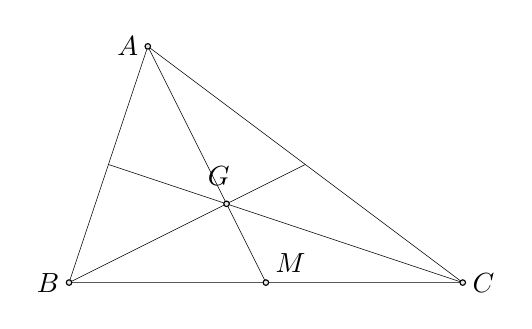
\begin{tikzpicture}
	\tkzDefPoints{1/3/A, 0/0/B, 5/0/C}
	\tkzDrawPolygon(A,B,C)

	\tkzCentroid(A,B,C)\tkzGetPoint{G}
	\tkzDrawLines[add = 0 and 1/2](A,G B,G C,G)

	
	\tkzInterLL(A,G)(B,C) \tkzGetPoint{M}
	\myShowPoints{M}{above right}
	\myShowPoints{A,B}{left}
	\myShowPoints{C}{right}
	\myShowPoints{G}{xshift = -.1 cm, yshift =.6cm}
\end{tikzpicture}
\end{document}